
\documentclass[conference]{IEEEtran}
\usepackage{blindtext}
\usepackage{multirow}
% tabularx allows manual tweaking of column width
\usepackage{tabularx}
% longtable does better format for tables that span pages
\usepackage{longtable}
\usepackage{hyperref}
\usepackage{amsfonts,amsmath,amssymb,graphicx,url}
\usepackage[noadjust]{cite}
% numeric is about equal to Bibtex's plain
\usepackage[english]{babel}
\usepackage{graphicx}
\usepackage{subcaption}

\hypersetup{
    colorlinks=true,
    linkcolor=blue,
    filecolor=magenta,
    urlcolor=cyan,
}
\usepackage{booktabs}
\usepackage{multirow}
\usepackage{tabularx,ragged2e}
% \newcolumntype{L}{>{\Left\arraybackslash}X} % centered "X" column
\newcolumntype{L}[1]{>{\raggedright\let\newline\\\arraybackslash\hspace{0pt}}m{#1}}

\usepackage{ amssymb }
\usepackage{graphicx}


\ifCLASSINFOpdf

\else

\fi

\hyphenation{op-tical net-works semi-conduc-tor}



\begin{document}
%
% paper title
% can use linebreaks \\ within to get better formatting as desired
\title{Report for CSE 505 - Phase 3}


% author names and affiliations
% use a multiple column layout for up to three different
% affiliations
\author{\IEEEauthorblockN{Xiaofei Sun}
\IEEEauthorblockA{Stony Brook University\\
ID:111753600\\
Email: http://www.michaelshell.org/contact.html}
}

\maketitle


\begin{abstract}
%\boldmath
My abstract
\end{abstract}

\begin{IEEEkeywords}
Multi-valued Real Logic, Tensor Network, Reasoning.
\end{IEEEkeywords}



% !TEX root = main.tex

\section{Paper Overview}

\subsection{Basic Information}

Here is some basic information about the paper I selected:

\begin{itemize}
    \item Title: Logic Tensor Networks: Deep Learning and Logical Reasoning from Data and Knowledge\cite{serafini2016logic}.
    \item Author: Luciano Serafini and Artur d’Avila Garcez
    \item From: ArXiv.2016
    \item Abstract: This paper proposes Logic Tensor Networks (LTN) to integrate \textbf{learning} and \textbf{reasoning} together based on vector representation. The proposed model LTN represent each object with a vector and then converts each function on multiple objects into a manipulate on their vector representations. Then it also uses a s-norm operator to transform a predicate to a real number in $[0,1]$, which means the confidence of this predicate. Finally, it defines a lose function for all predicates, which means it transfers the reasoning process into a learning and optimization problem.
\end{itemize}

\subsection{Definitions}

Recall that a first-order language $L$ is composed by three parts:
\begin{itemize}
    \item $\mathcal{C}=\{c_1,c_2,\dots\}$, the set of constant symbols;
    \item $\mathcal{F}=\{f_1,f_2,\dots\}$, the set of functional symbols;
    \item $\mathcal{P}=\{p_1,p_2,\dots\}$ the setof predicate symbols.
\end{itemize}


\subsection{Groundings}

LTN defines a term $\mathcal{G}$, called \textbf{grounding}, which contains $\mathcal{G}(c)$, $\mathcal{G}(f)$, $\mathcal{G}(P)$ respect to $c \in \mathcal{C}$, $f\in \mathcal{F}$, $P \in \mathcal{P}$:

Also, LTN define the manipulate of each clause $\phi$.

\subsubsection{Constant}
For each constant, LTN allocate a $n$-dimension vector to it:

\begin{equation}
    \mathcal{G}(c) \in \mathbb{R}^n
\end{equation}

\subsubsection{Function}

For each function $f/m$ on $m$ parameters, LTN define it as a mapping on vector space, which means:

\begin{equation}
    \mathcal{G}(f(t_1,t_2,\dots,t_m)) \in \mathbb{R}^{mn}\rightarrow \mathbb{R}^n
\end{equation}

Note that here we specify the parameter of $f$ is $t_i$ instead of $c_i$ because function $f$ can be recursive like $f(f_1(c1,c2),f_2(c1,c3)$.

\begin{equation}
    \mathcal{G}(f(t_1,t_2,\dots,t_m))=\mathcal{G}(f)\mathcal{G}(t_1),\mathcal{G}(t_2),\dots,\mathcal{G}(t_m)
\end{equation}

More specifically, $\mathcal{G}(f(t_1,t_2,\dots,t_m))$ is fitted by a linear function, which can be implemented with tensor network:

\begin{align}
    \mathcal{G}(f(t_1,t_2,\dots,t_m)) =&\mathcal{G}(f)(v_1,v_2,\dots,v_m) \nonumber\\
    =&\mathcal{G}(f)(v) \nonumber\\
    =&M_f v+N_f
\end{align}

where $v=\left< v_1,v_2,\dots,v_m \right>$, $M_f \in \mathbb{R}^{n\times mn}$, and $N_f \in \mathbb{R}^{n}$

\subsubsection{Predicate}

Like the grounding of a function,

\begin{equation}
    \mathcal{G}(P(t_1,t_2,\dots,t_m)) \in \mathbb{R}^{mn}\rightarrow [0,1]
\end{equation}

Again, as $t_i$ has been mapped to a vector, then:

\begin{equation}
    \mathcal{G}(P(t_1,t_2,\dots,t_m))=\mathcal{G}(P)\mathcal{G}(t_1),\mathcal{G}(t_2),\dots,\mathcal{G}(t_m)
\end{equation}

Therefore we transfer a predicate into a series of manipulation on tensor space:

\begin{align}
    \mathcal{G}(P(t_1,t_2,\dots,t_m))=&\mathcal{G}(f)(v_1,v_2,\dots,v_m) \nonumber \\
    =&\mathcal{G}(f)(v) \nonumber \\
    =&\sigma(u_p^T tanh(v^{T} W_{P} v +V_Pv+B_P))
\end{align}

where $v=\left< v_1,v_2,\dots,v_m \right> \in \mathbb{R}^{mn} $, $W_P \in \mathbb{R}^{mn \times mn \times k}$, $V_P \in \mathbb{R}^{mn \times k}$, $B_P \in \mathbb{R}^{k}$, $u_P \in \mathbb{R}^{k}$, and $\sigma$ is the sigmoid function.

\subsubsection{Clause}

In this project, we assume each clause is disjunctive normal form. So it's easy to get that

\begin{equation}
    \mathcal{G}(\phi_1, \phi_2, \dots, \phi_k)=\mu(\mathcal{G}(\phi_1),\mathcal{G}(\phi_2),\dots,\mathcal{G}(\phi_k))
\end{equation}

where $\mu$ is the max function.

\subsection{Optimization}

So now we get the definition of all components of multi-valued first-order language in tensor networks. The next step is to define a proper lose function.

Saying we know the value of $\phi(x)$ in our dataset, where $x$ is a constant. Intuitively, an optimal grouding should make $\mathcal{G}(\phi(t))$ as close as to $\phi(x)$.


% !TEX root = main.tex

\section{Models}

\subsection{Logic Tensor Network (LTN)}

multilayer perceptron (MLP). The key differencen is that the first layer is not linear layer but bilinear layer.

\begin{figure}
    \centering
    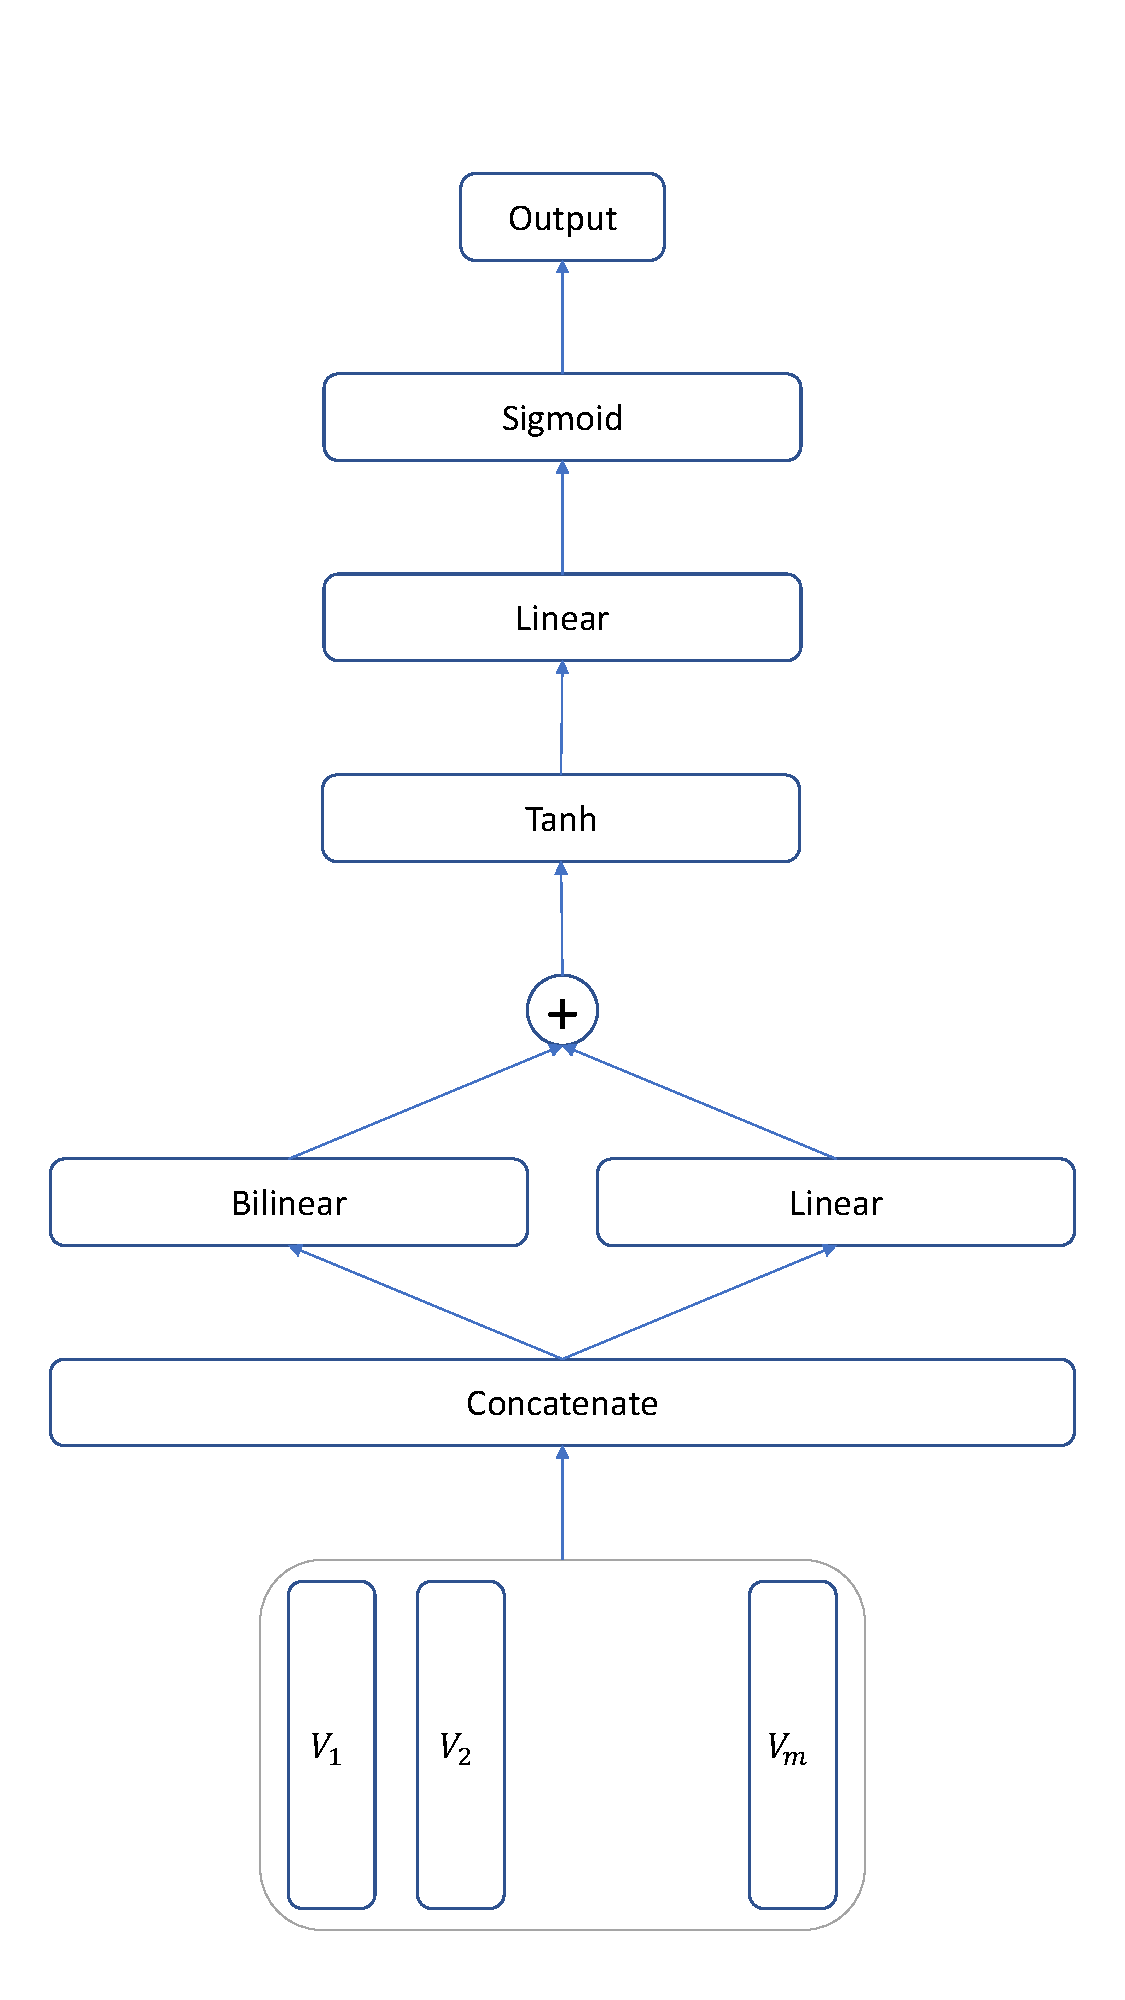
\includegraphics[width=.4\textwidth]{img/Predicate.pdf}
    \caption{Model for Predicate}
    \label{fig:LTN_predicate}
\end{figure}

\subsection{Convolutional Logic Tensor Network (CLTN)}

The model in original LTN is based on classical neural networks. However, recent development on deep learning shows that convolutional neural network (CNN) has more powerful ability. That makes us to extend LTN with CNN.

Here we first follow up the implementation of $G(c)$, $G(f)$, and $G(\phi)$. However, we tend to use Convolutional Neural Network to implement $G(p)$.

First we need to construct the input matrix with the $v_1,v_2,\dots,v_m$. From LTN model, we learned that the bilinear manipulation is critical to get a good performance. Here we construct this bilinear function directly using input vectors of constants. That is, suppose we get $m$ vectors called $x=[v_1,\dots,v_m]$, then $x\in \mathbb{R}^{k\times m}$, where $k$ is the dimension of constant vectors. Therefore, $x^Tx \in \mathbb{R}^{m\times m}$ a squre matrix, which can be treated as a 1-channel image.

The following step is trivial and the model is illustrated in Figure \ref{fig:CLTN_predicate}

\begin{figure}
    \centering
    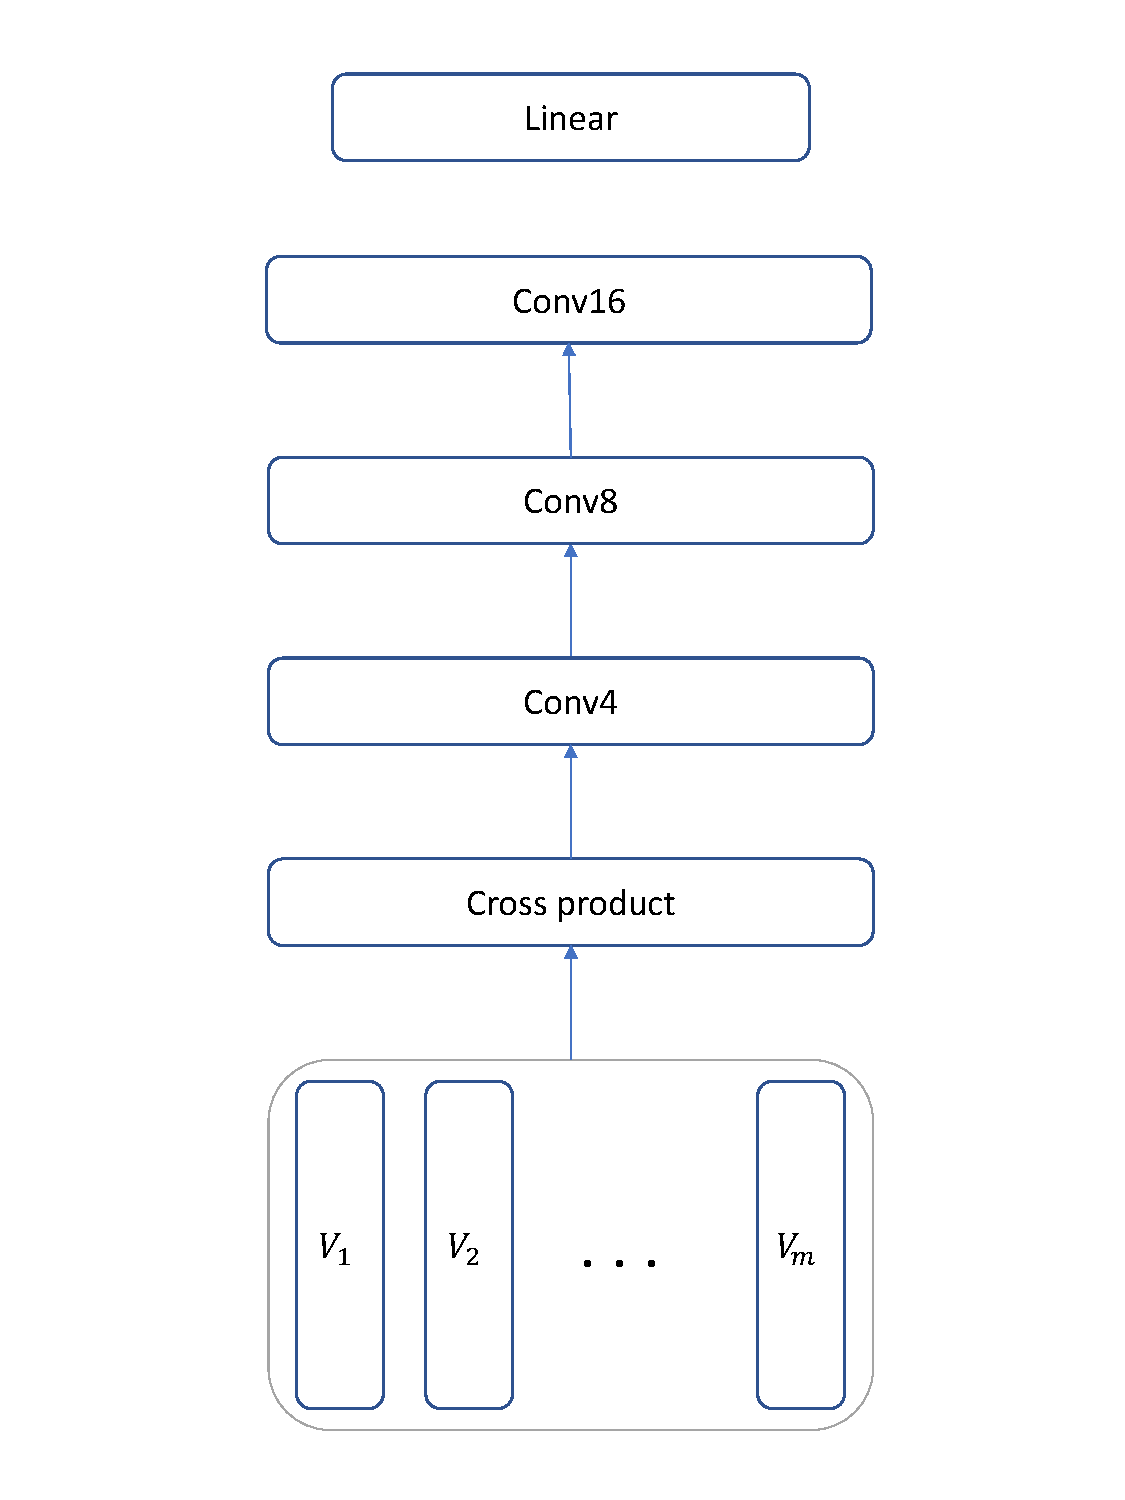
\includegraphics[width=.4\textwidth]{img/CLTN_Predicate.pdf}
    \caption{Model for Predicate}
    \label{fig:CLTN_predicate}
\end{figure}

\subsection{Universal and Existential Quantifiers}

One of the most difficult part of LTN is how to solve universal and existential quantifiers. In our implementation, we generated all the possible clause of a propositional by enumerating all variables.

For universal quantifier, the generated result is a set of clauses, while the result of existential quantifier is one clause. For example, given two propositionals $\forall \neg F(x, x)$ and $\exists y F(a,y)$, if $x,y \in {a,b,c}$, then we can get the corresponding results as $\{F(a,a),F(b,b),F(c,c)\}$ and $F(a,a)\vee F(a,b) \vee F(a,c)$

\subsection{Weighted Knowledge Base}

As we said before, we generated all possible clauses. However, such generated clauses could be even more than the observed knowledge base, which would potentially caused the overfitting on generated knowledge base and underfitting on observed knowledge base.

To solve this problem, we add a weight to each generated clause and confine that the sum of weights of clauses generated by the same propositional should equal to 1. In another word, if the generated clauses of $\phi$ is $\{\phi_1,\phi_2, \dots, \phi_n\}$, then the weight for each $\phi_i$ should be $\frac{1}{n}$.


% !TEX root = main.tex

\section{Experiments}

\subsection{Fit Knowledge Base}


\begin{figure*}
    \centering
    \begin{subfigure}[b]{0.3\textwidth}
        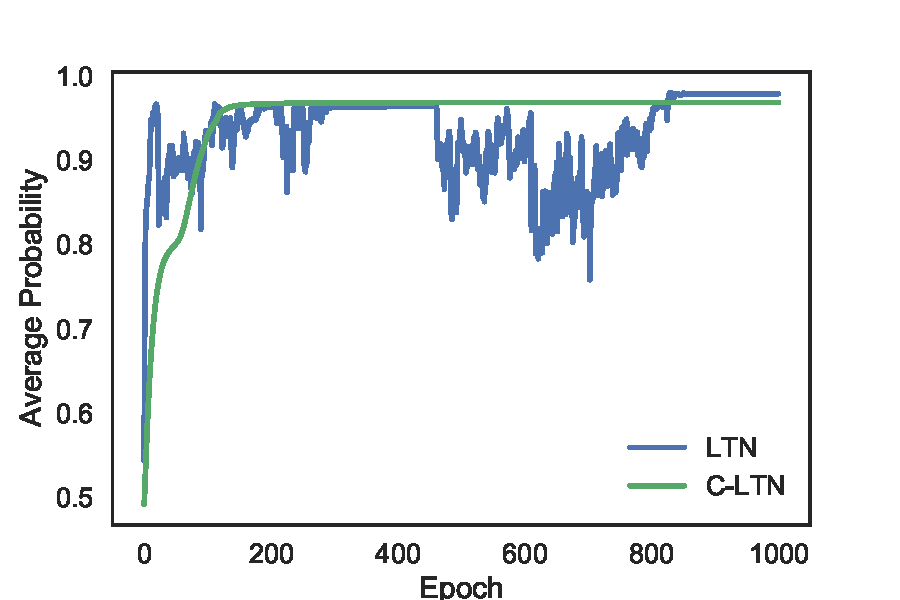
\includegraphics[]{img/curve1}
        \caption{A gull}
        \label{fig:gull}
    \end{subfigure}
    \begin{subfigure}[b]{0.3\textwidth}
        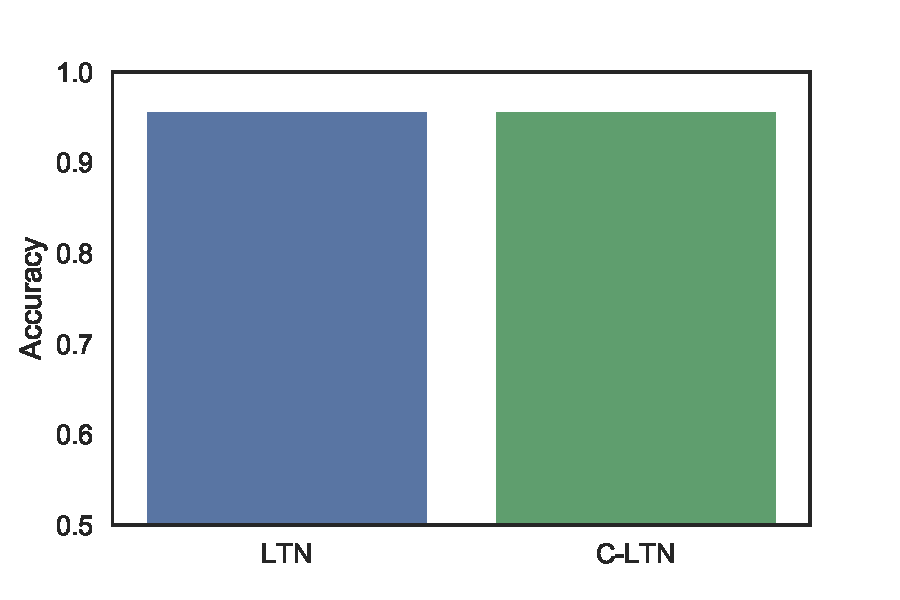
\includegraphics[]{img/bar1}
        \caption{A tiger}
        \label{fig:tiger}
    \end{subfigure}
    \begin{subfigure}[b]{0.3\textwidth}
        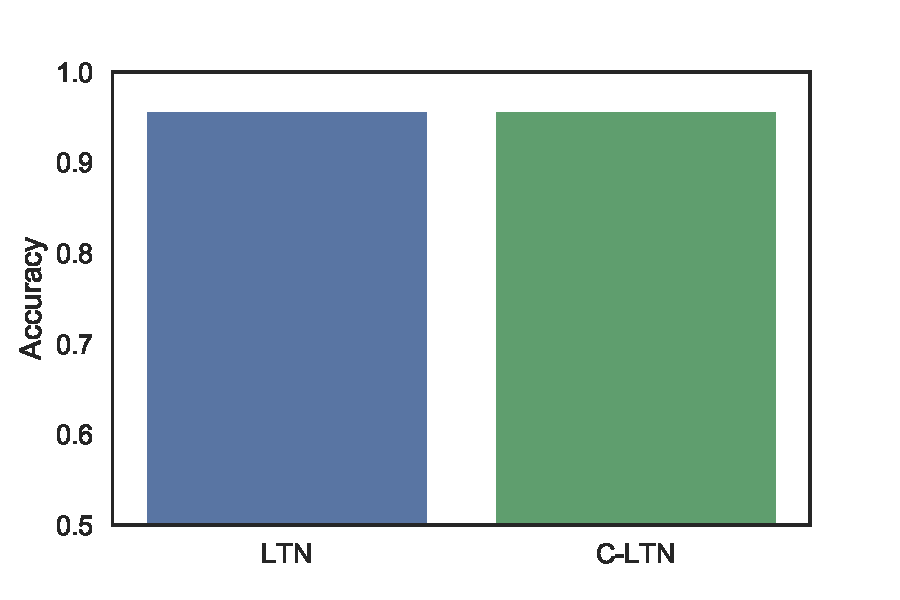
\includegraphics[]{img/bar1}
        \caption{A mouse}
        \label{fig:mouse}
    \end{subfigure}
    \caption{Pictures of animals}\label{fig:animals}
\end{figure*}

\subsection{Learn From Rule}

\subsection{Parameter Sensitive}


% !TEX root = main.tex

\section{Details and Discussion}



\bibliographystyle{IEEEtran}
\bibliography{reference}


\end{document}
